\chapter{Background}\label{chp:background} 
\chapterprecishere{"We model the future on the past. Sometimes that’s a mistake."\par\raggedleft--- \textup{Van Jacobsen}, SIGCOMM 2001}

This chapter will give a brief overlook of the motivation for \gls{ICN}, as well as explaining more details of the \gls{ICN} protocol \gls{NDN}.
The \gls{NDN} architecture will be reviewed.
Finally there will be a quick summary of related work to this thesis.

\section{Motivation for Information-Centric Networking}
When Internet was created in the 1960s', the researchers where inspired by the existing communication network; the telecommunication network.
Because it was natural and logical to think that people would send and receive short messages and instructions, the point-to-point communication model was a logical architecture. 
As Internet has developed, the traffic has increased enormously over the past few years. 
In the Global Internet Phenomena Report 1H2014 done by Sandvine~\cite{gipr2014}, shows that close to 64\% of all \gls{IP} traffic in North America was Real-Time Entertainment streaming.
In~\autoref{fig:ip-traffic} it can easily be seen that most of the traffic is content download, and not communication as Internet originally was designed for.
With this in mind, the \gls{IP} architecture does not provide an efficient transport model for what we are actually using the network for.

\begin{figure}[ht]
  \centering
  \begin{subfigure}{0.5\textwidth}
    \centering
    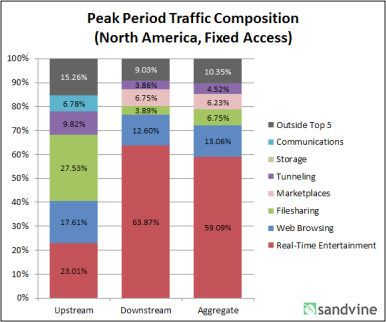
\includegraphics[width=0.98\linewidth]{north-america-ip-traffic.png}
    \caption{North America}
    \label{fig:north-america-ip-traffic}
  \end{subfigure}%
  \begin{subfigure}{0.5\textwidth}
    \centering
    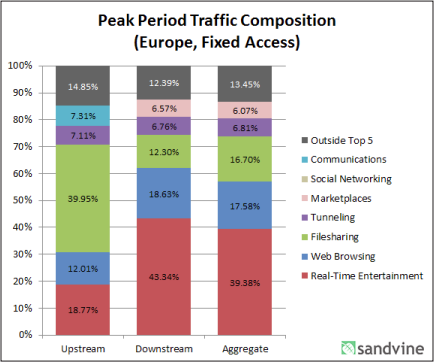
\includegraphics[width=0.98\linewidth]{europe-ip-traffic.png}
    \caption{Europe}
    \label{fig:europe-ip-traffic}
  \end{subfigure}
  \caption[Peak Period Aggregate Traffic Composition]{
  Peak Period Aggregate Traffic Composition in (a) North America and (b) Europe, fixed Access~\cite{gipr2014}.
  In North America, Netflix alone is responsible for 34.21\% of all content download.
  }
  \label{fig:ip-traffic}
\end{figure}

When designing the \gls{IP} network, security was not the first priority.
A logical thought considering that they did not know what the Internet is being used for nowadays and how big it has become.
Many protocols related to Internet has been designed and deployed mainly with the goal of functionality, not thinking about security.
In the years after the birth of Internet, it was discovered that Internet needed security at several layers, due to the increase of application requirements and transmission importance.
\gls{IPsec} is a very good example of work trying to patch up security flaws in the design of Internet.

Today, WiFi is disseminated across homes and buildings in many countries. 
Wireless technology has grown rapidly and it is predicted continuous growth in the years to come~\cite{DBLP:journals/jthtl/Rosston14}. 
The \gls{IoT} trend is coming and the \gls{IP} network is not designed for broadcast.
Therefore wireless connection is not as easy as it should and could be.
Devices should easily be able to communicate directly with each other without having to interconnect through a router.

Another problem is the network redundancy. 
Looking at~\autoref{fig:ip-traffic} and reading~\cite{gipr2014} where it comes to light that Netflix stands for 34.21\% of all content download in America, one can conclude that there are a lot of movies downloaded from \textit{x} users geographically located close.
And thus the network path from the source (e.g. Netflix) to this geographical place is allocated \textit{x} too many times. 
This is because a node in an \gls{IP} network does not know \textit{what} it processes, but rather the packets' endpoints, i.e. \textit{where} it goes and \textit{where} it comes from, hence the node throws all packets after use. 
The fact the every node knows nothing about the content the process, makes every node dumb.
The network is designed for redundancy when it comes to content download.

These design failures are some the reasons why the research for the future Internet began.  
\gls{ICN}~\cite{DBLP:journals/cm/AhlgrenDIKO12} is a concept developed under this research.
It is built upon delivery of content, rather than the point-to-point model we previously have seen in \gls{IP}.
\gls{ICN}s goal is to build an infrastructure of a new Internet that can achieve efficient, secure and reliable distribution of content.
In 2012 \gls{IRTF} established \gls{ICN} working group.


\section{Content Centric Network \& Named Data Network}\label{chp2:sec:icn}
The first network protocol purposed for \gls{ICN}, \gls{CCN}, was presented by Van Jacobsen at a Google Talk in 2006. 
He, amongst other contributors of \gls{CCN}, has been working on developing the Internet as we know it since the early start.
Jacobsen has contributed to \gls{TCP}/\gls{IP} with his flow control algorithms~\cite{DBLP:conf/sigcomm/Jacobson88} and \gls{TCP} header compression~\cite{rfc1144}.
\gls{CCN} focuses on naming content, instead of naming \gls{IP}-addresses. 
The research project is lead by \gls{PARC}.
A branch of \gls{CCN} is the \gls{NDN}~\cite{DBLP:journals/ccr/0001ABJcCPWZ14} research project started in 2010, which Jacobsen also have contributed to.
One of the biggest contributers is \gls{UCLA}, with Lixia Zhang in the lead. 
Zhang is known for her contribution to, amongst many other, \gls{RSVP}~\cite{rfc2205} and \gls{MACAW}~\cite{DBLP:conf/sigcomm/BharghavanDSZ94}.
The \gls{NDN} project is also one of few projects funded by \gls{NSF} in their \gls{FIA} program~\cite{nsf-fia}.

\section{NDN Architecture}\label{chp2:sec:ndn_architecture}
Since the knowledge of how \gls{NDN} works is not disseminated amongst computer scientists, it is essential for this thesis to describe how it works.
This section will describe the basic architecture of \gls{NDN}~\cite{NDN-0021} and compare some solutions with the equivalent solutions in \gls{IP}.

\subsection{Brief Introduction}
In \gls{NDN} there are two types of packets, \gls{interest} and \gls{data} packet.
All \gls{data} has be given a content \gls{name} by its \gls{publisher}. 
To publish some content to the network, a user have to register the prefix, i.e. announcing the contents \gls{name}, which tells the network that the content can be retrieved on the announced \gls{name}. 
The retrieval can only be achieved if someone expresses an \gls{interest} to the content \gls{name}.
If a user expresses \gls{interest} in the \gls{name}, the network will route the \gls{interest} to the closest \gls{node} that holds the \gls{data}. 
The \gls{data} packet can be retrieved from any \gls{node}, trusted or not, over any type of communication channel, secure or not. 
This is due to that the network layer demands a signature from the content's \gls{publisher}.
Finally the \gls{requester} will receive the \gls{data} packet containing the content requested.
The \gls{data} can be verified by the requester ensuring that the \gls{publisher} who ``owns'' the content actually is the owner, because its cryptographically signed.
If confidentiality is needed, the \gls{data} can be encrypted, thus the communication channel does not need to be secured. 

A \gls{NDN} node is slightly different to an \gls{IP} node. 
Since the \gls{data} is linked to a \gls{name} and signed by its \gls{publisher}, the node can cache the \gls{data} and be able to satisfy other \texttt{Interests} to the same \gls{data}. 
This provides natural \gls{multicast} in the network, and will ease the network load drastically.

Securing the \gls{data} rather than the connection, leads to a network where one can easily verify the connection between content and its \gls{publisher}.

\subsection{NDN - Based on Existing Concepts}
The goal for the network design is essentially making it more secure and applicable for content without removing the communication service that \gls{IP} was designed for. 
Designing a new network protocol we have to look at what measurements have been done in the existing \gls{IP} network to tailor it towards content sharing.
As the reader might notice after reading the background material, \gls{NDN} is built upon concepts that we can map to well working solutions deployed over \gls{TCP}/\gls{IP}.
Some examples are:
\begin{itemize}
  \item BitTorrent - 
  The concept of sharing bits of files between peers in a network is a well-working distributed method for sharing content. 
  Requesters does not care where the content come from, but only that the content is what is requested.
  \item \gls{CDN} - 
  Many \gls{ASP}s, such as Netflix and YouTube, have found out that their service performs a lot better for their costumers if they cache up their data close to where the users is located.
\end{itemize}

\subsection{Packets}\label{packets}
There are two types of packets in \gls{NDN};
\textit{\gls{interest} packet} and the corresponding answer, i.e. the \textit{\gls{data} packet}, illustrated in~\autoref{fig:packets}.

\begin{figure}[H]
  \centering
  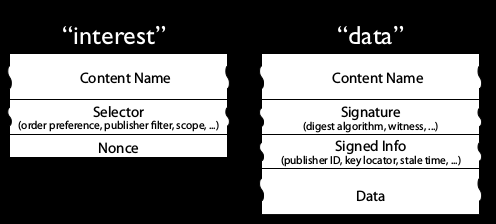
\includegraphics[width=1\textwidth]{packets.png}
  \caption[NDN packets]{\gls{interest} packet and \gls{data} packet.
  Reconstructed from~\cite{jac09-03}.
  }
  \label{fig:packets}
\end{figure}

The \gls{interest} packet specifies a content \gls{name}. 
The \gls{name} can have a hierarchical structure and signatures can be added after the \gls{URI}, e.g. ``/ndn/no/ntnu/haakon/file/1/<signature>''.
An \gls{interest} can also contain a set of different Selectors to specify original requirements for the \gls{data} response. 
Some of the Selector fields are:
\begin{itemize}
  \item KeyLocator - can be used to specify where the Public Key for the signature can be found.
  \item Exclude - can be used to specify a list or a range of names that should be excluded from the \gls{name}. 
  I.e. if the \gls{name} is ``/ndn/no/ntnu'' and the Exclude contains ``/item'', the returned \gls{data} cannot contain ``/ndn/no/ntnu/item''.
  \item MustBeFresh - if True, a \gls{node} cannot answer with a \gls{data} packet where the FreshnessPeriod has expired.
  FreshnessPeriod is a time value of how long some \gls{data} is fresh.
  \item ChildSelector - can be used to select either the leftmost (least) or the rightmost (greatest) child, e.g. content version. 
  \item Min/MaxSuffixComponents - refers to \gls{name} components that occur in the matching \gls{data} beyond the prefix. 
\end{itemize}
The Nonce field sets automatically. 
This is used to uniquely identify an \gls{interest} and prevent looping in the network.

The \gls{data} packet is a response to the \gls{interest} packet, and contains the content \gls{name} and the Content itself.
It also has a MetaInfo field that is used to specify the FreshnessPeriod (milliseconds), ContentType and FinalBlockId. 
When somebody requests a file ``/ndn/no/ntnu/haakon/file/1'' with an \gls{interest}, the response will have the same \gls{name}, but also containing the file.

Because a \gls{data} packet can only exists if there is a corresponding \gls{interest}, \gls{NDN} is pull-based.
Hence unsolicited \gls{data} packets will be thrown away, i.e. there is no content in the network, that is not requested from someone.
This reduces unwanted traffic compared to \gls{UDP} in \gls{IP}, and minimizes the \gls{DoS} vulnerability drastically.

\subsection{Names}\label{name}
In todays Internet we are well familiar with the mapping of \gls{URL} and \gls{IP} addresses.
This mapping, done by the \gls{DNS}, eases the pain of remembering an \gls{IPv4} (32-bit) address and lately also \gls{IPv6} (128-bit) addresses.

In a \gls{NDN} network a \gls{node} does not have an address nor a \gls{name}.
The routing of packets is done by content lookup, rather than address lookup.
This means that all content in the network do have a \gls{name}.
When an \gls{interest} is sent, each \gls{node} asks the network: ``Where can I find \textit{a} node that can provide me with this content?''.

There is no strict rules for a \gls{name} in \gls{NDN}.
This means that a network \gls{node} only routes an \gls{interest} based on longest prefix match.
Naming is left to the application design, thus it can be customized for the applications best purpose.
However the network assumes hierarchical structured names, hence routing will perform better with a hierarchical \gls{name} design.

For the network to perform even better, the \gls{interest} can append some Selectors that can help the network to decide which \gls{data} to retrieve and where to route.
With Selectors a partially known \gls{name} can successfully retrieve the right \gls{data}.
E.g. when a user want to download the newest version of some content, lets say ``/ndn/no/ntnu/haakon/file/<version?>'', but do not know which version is the newest, the user can append a ChildSelector to choose the newest version, if several versions are offered.

The fact that \gls{data} has a \gls{name} makes \gls{SDSI} and \gls{IBC} highly applicable to \gls{NDN}.
Namespace-based trust was introduced in \gls{SDSI}~\cite{rivest1996sdsi}, binding names to public keys.
\gls{IBC} will be explained in detail in~\autoref{chp:ibc}, and is a key topic in this thesis.

\subsection{Network Node}
It may sound like a impossible task to force todays network from \gls{IP} to \gls{NDN}. 
But looking at history, \gls{IP} first ran over the telecommunication network and later established its own physical network, \gls{NDN} can run over the \gls{IP} network and later create its own physical network. 
Also, if we look at an existing model of an \gls{IP} node~\autoref{fig:ip-model-node} and compare it to a \gls{NDN} node~\autoref{fig:icn-model-node}, we see that they look much the same.
The only significant difference in hardware is the storing capacity, which becomes cheaper and cheaper each month.
However, the logic behind a \gls{NDN} \gls{node} is a bit more complex, and thus lead to more knowledge about \textit{what} content the node has to offer.
To understand this, the following entities in a \gls{NDN} \gls{node} should be understood:
\begin{enumerate}\label{ndn-node-modules}
  \item Face - A term used for generalization of different interfaces, e.g. physical like Ethernet, or overlay like \gls{TCP} and \gls{UDP}. A Face can also be a UNIX-domain socket for communication with a local application.
  \item \gls{PIT} - All pending or recently satisfied \gls{interest}s are stored here, together with the incoming and outgoing Face.
  If a new incoming \gls{interest} matches an entry in the \gls{PIT}, the incoming Face will be added to the entry. 
  \item \gls{CS} - When a \gls{node} receives a \gls{data} packet that has the corresponding entry in the \gls{PIT}, it stores the \gls{data} packet in \gls{CS} as long as possible. 
  The \gls{CS} works like a cache for the \gls{node}.
  \item \gls{FIB} - Forwarding strategy is stored for each \gls{name} prefix. 
  When a \gls{node} forwards an \gls{interest}, it will do a longest prefix lookup in the \gls{FIB} and send the \gls{interest} further to the best matching Face.
\end{enumerate}

\begin{figure}[H]
  \centering
  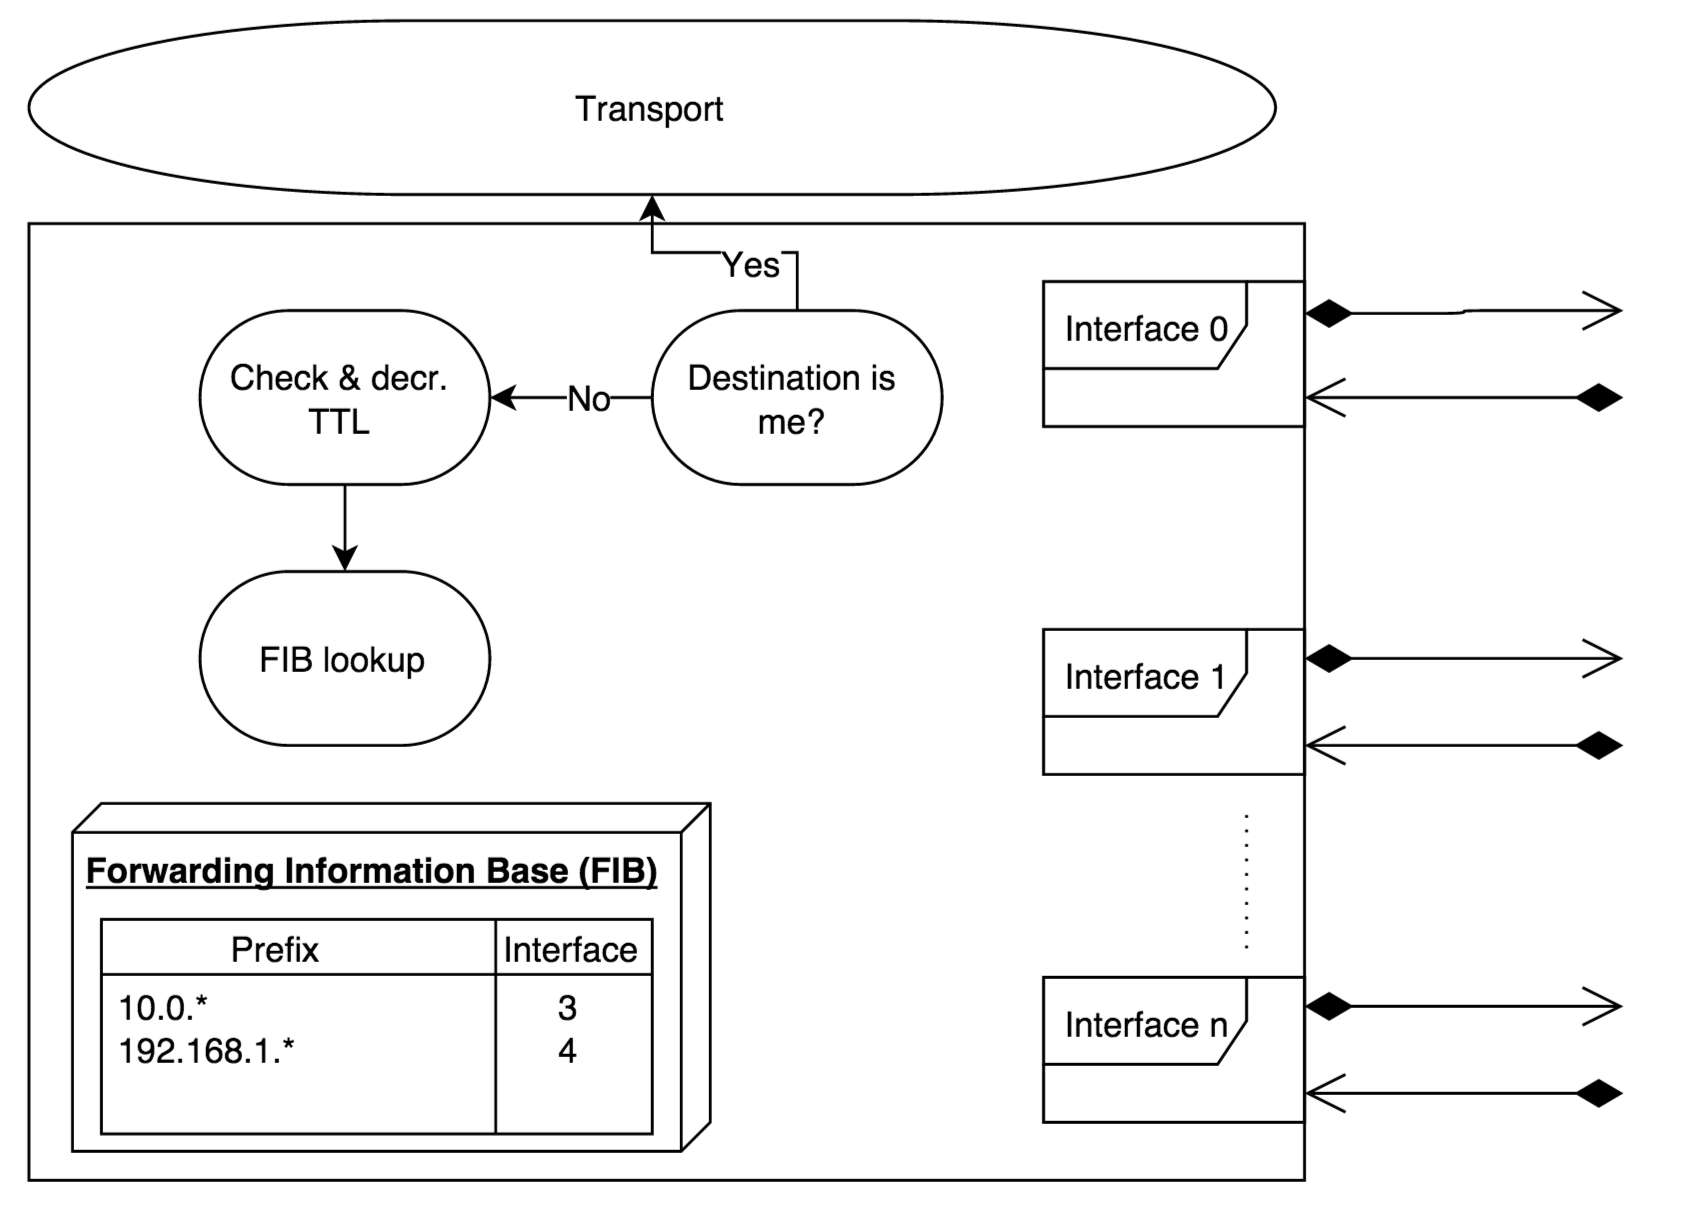
\includegraphics[width=0.8\textwidth]{ip_model_node.png}
  \caption[Model of IP node]{Model of IP node. A packets enters the node through an interface. 
  The node decides whether the packet is for the node itself, or passes it further to next node, found in the FIB.
  Reconstructed from~\cite{jac09-03}.}
  \label{fig:ip-model-node}
\end{figure}

\begin{figure}[H]
  \centering
  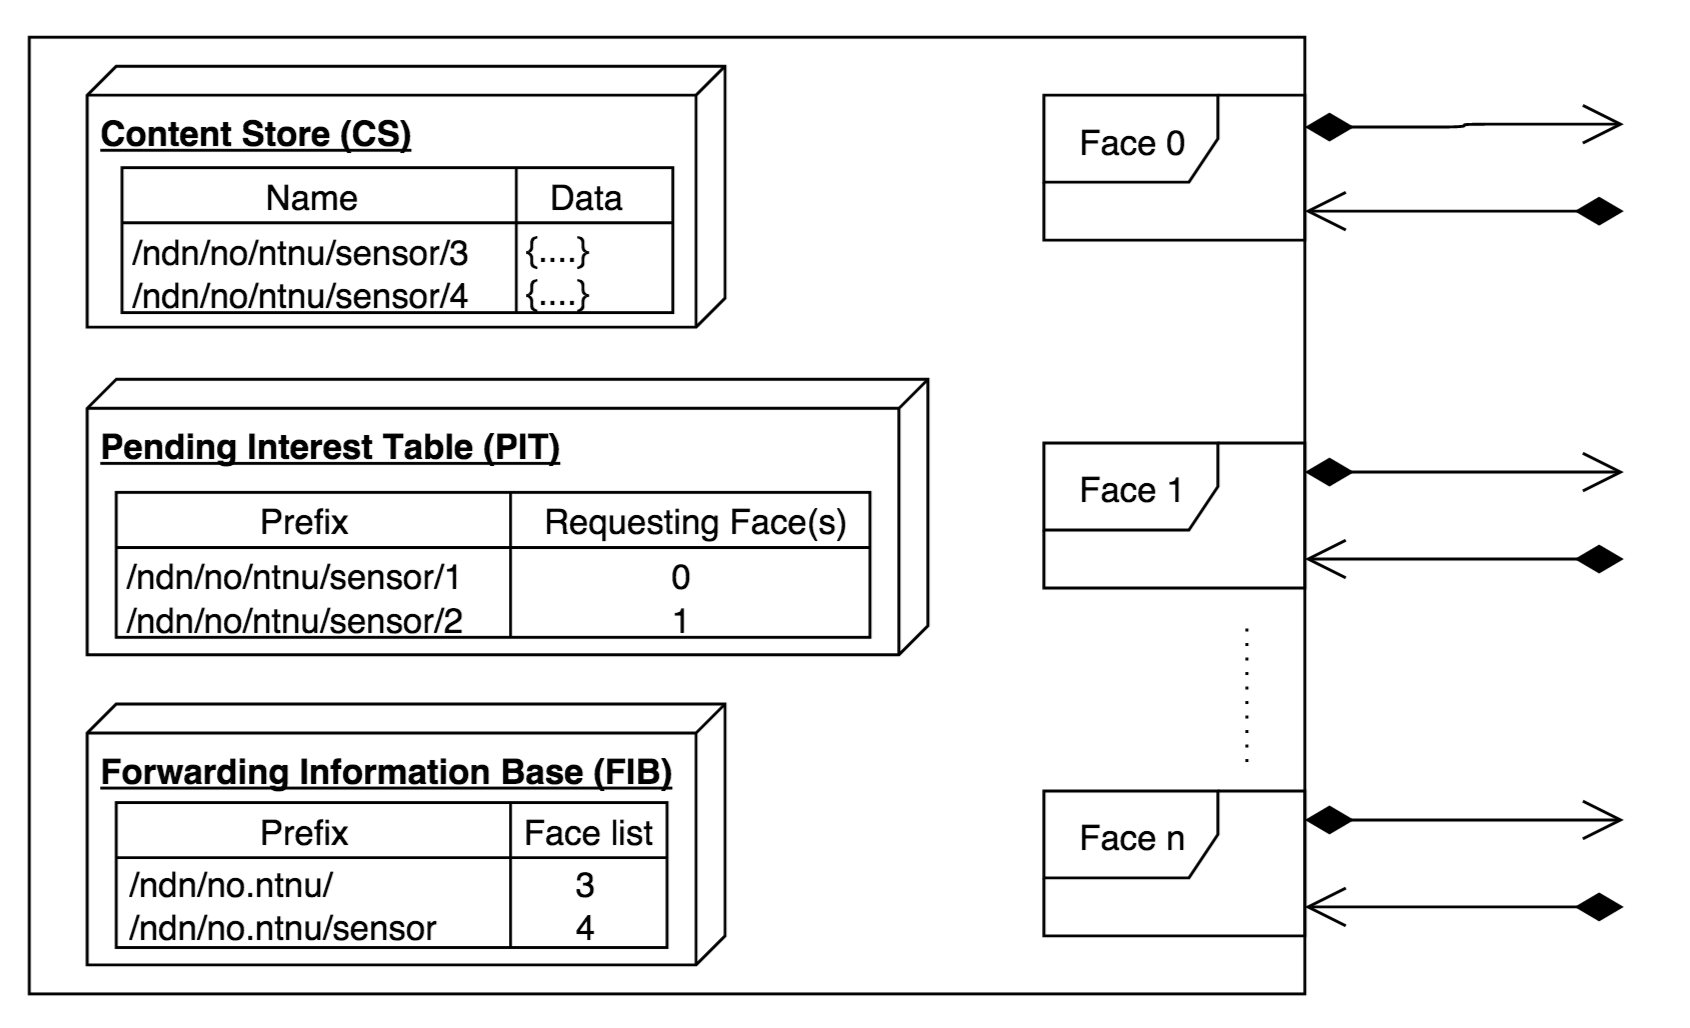
\includegraphics[width=0.8\textwidth]{icn_model_node.png}
  \caption[Model of NDN node]{Model of NDN node. A packet enters through an Face. 
  The node checks whether the \gls{interest} is already queried in the PIT, or stored in the CS, or passes it further to next node, found in the FIB.
  Reconstructed from~\cite{jac09-03}.}
  \label{fig:icn-model-node}
\end{figure}

In contrary to an \gls{IP} node, a \gls{NDN} node knows \textit{what} content comes through itself. 
Since all content is associated with a \gls{name}, a \gls{NDN} node can know 1) \textit{what} is requested, but not satisfied (i.e. stored in \gls{PIT}), and 2) \textit{what} has been satisfied earlier and still available, i.e. still cached in \gls{CS}.
With this knowledge the network can now satisfy \texttt{Interests} with content already stored in cache, hence the network can naturally offer \gls{multicast} on network layer.
~\autoref{fig:ndn-multicast} illustrates a \gls{NDN} network where we can see that the network does not nearly have to send equal amount of content than in an \gls{IP} network.
The mobile expresses an \gls{interest} (1) in a file named \path{/ntnu/file1}.
The \gls{interest} finds its way to the \gls{publisher} of the file, and thus the \gls{publisher} responds with a \gls{data} packet (2) named \path{/ntnu/file1} containing the file, and the \gls{data} finds it way back to the mobile.
When the second computer expresses the same \gls{interest} (3), the consecutive node has already cached the \gls{data} response matching to the \gls{interest} in its \gls{CS}, hence the \gls{interest} is satisfied already at this point (4), and not forwarded any further.
Same happens when the third computer expresses again the same \gls{interest} (5) to the network.
Given that the file (\path{/ntnu/file1}) these computers are interested in is 4 gigabyte, the network saves a lot of traffic with \gls{multicast} provided by \gls{NDN}.
Best case scenario in \gls{NDN} is illustrated in~\autoref{tbl:node_comparison-ip-ndn}.
Every node is saving bandwidth in a \gls{NDN} network compared to nodes in an \gls{IP} network.
Worst case scenario, where cached \gls{data} is thrown away, the \gls{NDN} nodes will perform equal to the \gls{IP} nodes.

\begin{figure}[H]
  \centering
  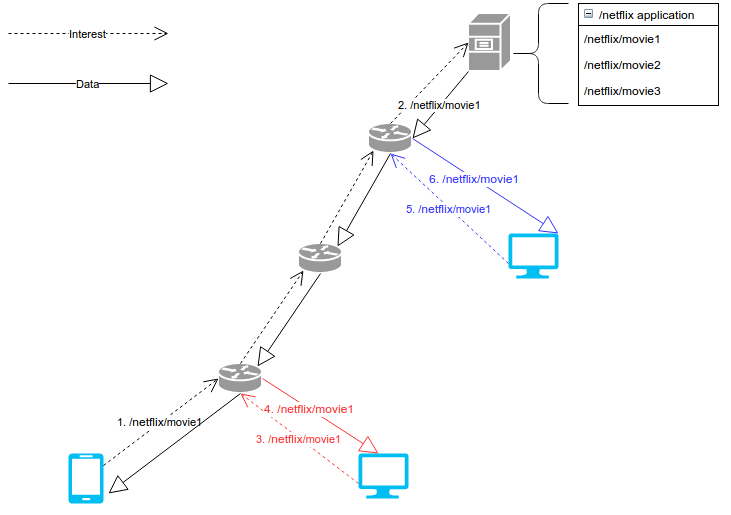
\includegraphics[width=1\textwidth]{ndn-multicast.png}
  \caption[Multicast in NDN]{Multicast in NDN.}
  \label{fig:ndn-multicast}
\end{figure}

\begin{table}[h]
  \begin{tabular}{llll}
  Node        & Data in/out IP  & Data in/out NDN   & \% bandwidth needed in NDN    \\ \hline
  node1       & 8GB/8GB         & 4GB/8GB           & 50\%/100\%      \\ %\hline
  node2       & 8GB/8GB         & 4GB/4GB           & 50\%/50\%     \\ %\hline
  node3       & 12GB/12GB       & 4GB/8GB           & 33\%/66\%     \\ %\hline
  Publisher   & -/12GB          & -/4GB             & -/33\%        \\ %\hline
  \end{tabular}
  \caption[Bandwidth comparison of NDN and IP]{Node bandwidth allocation comparison in IP and NDN (best case). Mobile, 2\textsuperscript{nd}device and 3\textsuperscript{rd}device requests \protect\path{/ntnu/file1} (4GB). The NDN nodes allocates bandwidth 44.3\% (incoming) and 66.3\% (outgoing) compared to IP nodes.}
  \label{tbl:node_comparison-ip-ndn}
\end{table}
 
\subsection{Incoming Interest}\label{incoming-interest}
In~\autoref{fig:icn-model-node-decision-interest} we see an incoming \gls{interest} through a Face. 
The node checks the \gls{PIT} for pending or recently satisfied \texttt{Interests}. 
If there is no match, the node will do a lookup in \gls{CS} to see if a corresponding \gls{data} packet is cached. 
If there is a match in the \gls{PIT} it will only add the Face to the \gls{PIT} entry. If there is a match in the \gls{CS} the node will return the \gls{data}. 
If there is no match in either the \gls{PIT} or the \gls{CS} the node will make a new \gls{PIT} entry and do a longest prefix match lookup in the \gls{FIB} to decide which Face(s) to forward the \gls{interest}.
The node waits for incoming \gls{data} and satisfies the \gls{PIT} entry when the \gls{data} arrives, explained in~\autoref{incoming-data}. 
Each \gls{PIT} entry has its own routing strategy. 
I.e. whether, when, and where to forward the \gls{interest}.
\begin{figure}[H]
  \centering
  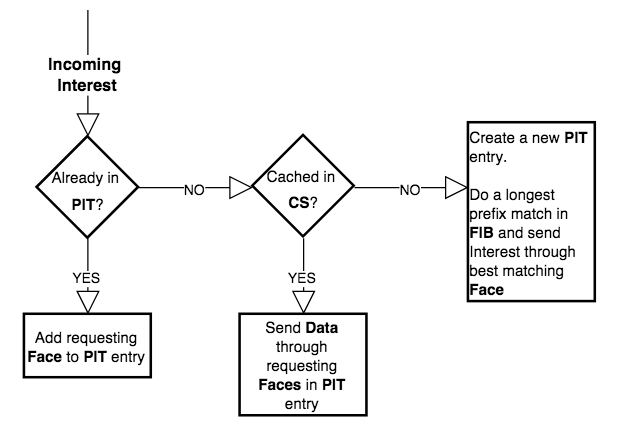
\includegraphics[width=1\textwidth]{ndn-node-decision-tree-interest.png}
  \caption[Incoming Interest - NDN node]{Decision tree for a NDN node when receiving an \gls{interest}.}
  \label{fig:icn-model-node-decision-interest}
\end{figure}

\subsection{Incoming Data}\label{incoming-data}
In~\autoref{fig:icn-model-node-decision-data} we see incoming \gls{data}.
The node will check  the \gls{PIT} for an entry, if a match is found the node will forward the \gls{data} to all the Faces registered in the \gls{PIT} entry.
If no match, the node will disregard the \gls{data} because it is unsolicited content.
The node checks the \gls{data} from local applications cached in \gls{CS} first, if there is no match, it stores the content in \gls{CS} and sends the \gls{data} to all requesters (i.e. through all Faces stored in the \gls{PIT} entry).
\begin{figure}[H]
  \centering
  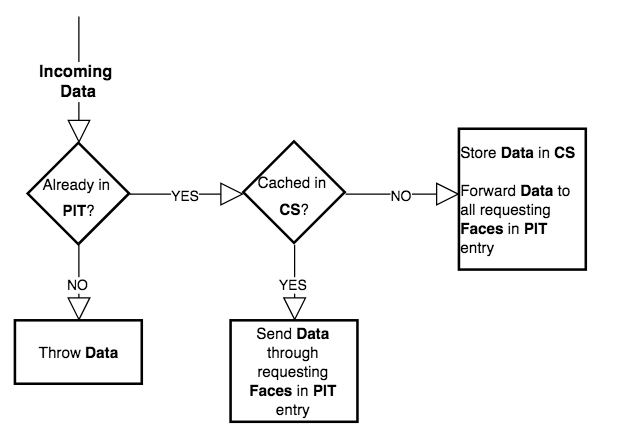
\includegraphics[width=1\textwidth]{ndn-node-decision-tree-data.png}
  \caption[Incoming Data - NDN node]{Decision tree for a NDN node when receiving \gls{data} packet.}
  \label{fig:icn-model-node-decision-data}
\end{figure}


\subsection{Security}\label{ndn-security}
Below I will present why \gls{NDN} facilitates good security properties, explaining some of the security aspects around \gls{NDN} discussed in~\cite{secure-network-content}, and the difference in securing data and securing channel.

\subsubsection{Trusting Host versus Trusting Content}
Doing a whole lot of mapping at different layers is not a good security model.
Each mapping introduces a potentially vulnerable target for forgery.
The \gls{IP} network is designed in a way that makes us want to trust the host.
What we are actually trusting is the mapping of the \gls{URL} to the \gls{IP} address.
\gls{DNS} points to a host address that speaks for the \gls{URL} you are interested in, and thus if someone manages to forge this address exploiting \gls{dnssec}, you cannot tell if you talk to the right host.

As seen in~\autoref{fig:ndn-vs-ip-architecture} the security in \gls{NDN} is dealt with in one layer, rather than over several layer as needed in the \gls{IP} architecture, i.e. \gls{TLS}, \gls{dnssec}, \gls{IPsec}, etc.
\begin{figure}[ht]
  \centering
  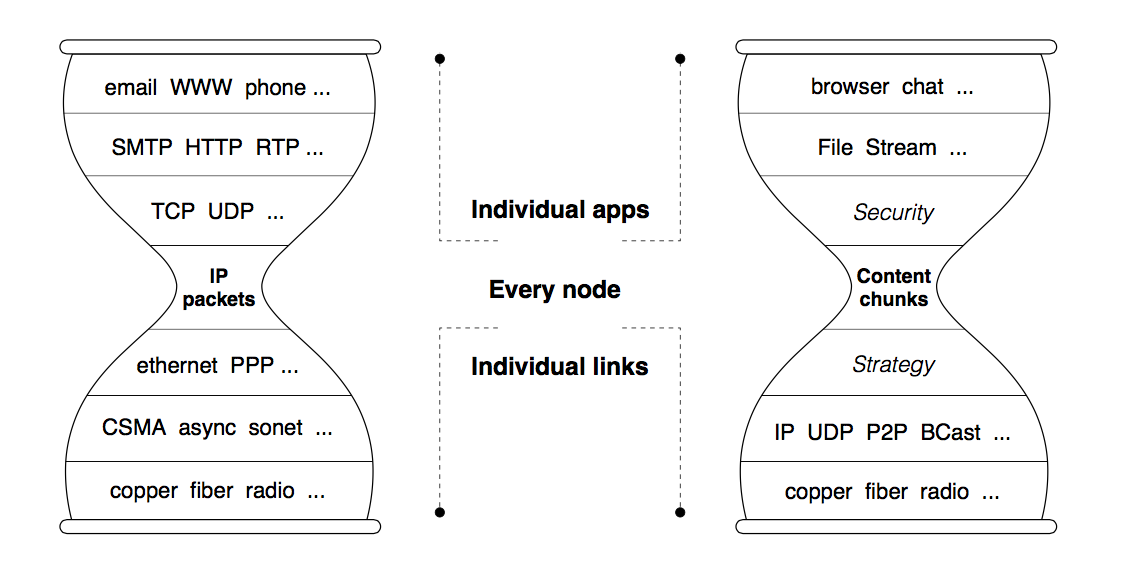
\includegraphics[width=0.7\textwidth]{ndn-vs-ip-architecture.png}
  \caption[NDN versus IP architecture]{NDN versus IP architecture. 
  The building blocks of the NDN architecture are named content chunks, in contrast to the IP architecture's fundamental unit of communication, which is a point-to-point channel between to endpoints identified by IP addresses.
  ~\cite{DBLP:journals/ccr/0001ABJcCPWZ14}.
  }
  \label{fig:ndn-vs-ip-architecture}
\end{figure}

The content is rarely encrypted and the confidentiality is not preserved, unless there is established a secure channel using e.g. \gls{TLS}.
This is a problem due to the issues concerning tampering and eavesdropping.
The content the host we trust provides can contain malicious software and important information can be swapped even though the channel is secured.
This is the concept of securing the channel, and the trust is based on certificates.
This trust is an issue itself. 
Due to the global \gls{PKI} and essentially because the certificate is signed by a \gls{TTP} all trust comes outside the namespace.
This makes it problematic to retrieve content over \gls{IP} from other sources than the trusted host because you do not trust any other than the host you are connected to via the secure channel.
The host does not provide any assurance that the content is verified by the host itself, it only assures a secure channel.

A goal is to get the desired content from the intended source, unmodified in transit.
Therefore a better solution would be to trust the content rather than the \gls{host} of the content.
This concept requires us to change the network trust.
Skipping 1) all the trust based in mapping of hosts, 2) where the data comes from, and 3) securing the channel.
The content should be linked to the \gls{publisher} and this linkage should be signed by the \gls{publisher}. 
The concept is to mathematically prove that the content originates from the believed \gls{publisher}, and that its not modified nor been exposed to unauthorized parties (if necessary).
This introduces a possibility that anyone can retrieve any piece of data from anyone, trusted or not, regardless of secure channel or not.
The question is how can this idea be achieved? 
As Diana Smetters and Van Jacobsen says~\cite{secure-network-content}, we must ensure the contents' validity, provenance and relevance.

\begin{itemize}
  \item Validity - Complete and unmodified content from the \gls{publisher}.
  \item Provenance - Should the \gls{publisher} be trusted with the content requested?
  \item Relevance - Is the content what the requester intended?
\end{itemize}

There exist concepts to achieve these goals.
One can do hash verification on the content to be sure that the content is unmodified. 
But there should also be a binding between the \gls{name} to the content.
However, this does not provide provenance nor relevance because the \gls{publisher} is not linked to the data, and thus we cannot be sure the \gls{publisher} knows what the content contains.
Hence there should be a linkage between the \gls{publisher}, the \gls{name} and the content.
A solution is to do a triple mapping of the \gls{name} (N) and content (C), cryptographically signed by the \gls{publisher} (P) seen in~\autoref{eq:mapping_name-content}.
This mapping is unique, relying on the hash computation done in the signing, providing validity, provenance and relevance.
A requester can easily verify the \gls{name} and content binding, as well as authenticating that the data originates from the \gls{publisher} who knows what the content is.
Anybody can retrieve \texttt{M\textsubscript{(N,P,C)}} and verify the content and publisher mapping, hence an untrusted \gls{host} and an insecure channel is not so bad anymore.

\begin{equation}\label{eq:mapping_name-content}
M_{(N, P, C)} = (N,C,Sign_{P}(N,C))
\end{equation}

A clear benefit of this approach is that it scales. 
The \gls{name} can be of any form because of the nature of hashing. 
Different naming rules should apply for different applications as there are no global naming rules that are optimal for each application.

This concept is integrated in the \gls{NDN} protocol and it is required that every packet delivered from application layer is signed by the application.
The protocol also provides an easy way for the application to encrypt data providing confidentiality.
Encrypting the content with symmetric keys that are distributed to parties obtaining access right to the content together with the validity, provenance and relevance provides a way of securing data rather than securing communication channels.

\subsubsection{Anonymity}
% TOR network
Based on the nature of this architecture, \gls{NDN} facilitates the practice of anonymity in the network. 
In a Tor network~\cite{DBLP:conf/uss/DingledineMS04}, each node participating in a circuit only knows the two neighboring nodes.
Only a \gls{gpa} that can monitor the entire network is able to decide the whole packet path, hence an adversary can know \textit{who} is requesting and \textit{who} is responding.
Since the packet format (\autoref{packets}) in \gls{NDN} has no source or destination specific field as in a \gls{IP} packet, the privacy of the network is more similar to a Tor network.
If a packet is captured at any arbitrary point of its path, the only information an adversary will get, is the two nodes between the packet capture and the content \gls{name}. 
Unless monitoring a complete network, it should be close to impossible to track packets.  
However, because of the semantic naming there are some issues related to privacy as it easily can be seen in the \gls{name} \textit{what} the content contains in many cases.
Also since signing of each \gls{interest} is required by the sender, some privacy information might leak.
DiBenedetto et al. try to address these problems in~\cite{DBLP:conf/ndss/DiBenedettoGTU12} with an approach that use existing solutions from the Tor network.
In 2010 the \gls{NDN}-team planned to implement TORNADO~\cite[Section 3.7]{NDN-0001}, the \gls{NDN} version of Tor, to demonstrate the privacy preservation capabilities of the network.

\section{Attacks}

Paolo Gasti et al. identifies several \gls{DoS} attacks on \gls{NDN} in their paper about \gls{DoS} and \gls{DDoS} in \gls{NDN} ~\cite{DBLP:conf/icccn/GastiTU013}. 
Other works have been done related to \gls{DoS} in \gls{NDN}~\cite{DBLP:journals/ijcomsys/WangCZQZ14, DBLP:conf/ancs/SoNO13, DBLP:journals/corr/abs-1303-4823}

In~\cite{DBLP:journals/tifs/LiZZSF15} Zhang et al. propose an extension of the \gls{NDN} protocol for addressing the access problem of cached \gls{data} in nodes.  
The \gls{NDN} network is also potentially susceptible to content poisoning attacks which Ghali et al. addresses in~\cite{DBLP:journals/ccr/GhaliTU14}.

\section{Related work}
The work in this thesis builds upon three main concepts: synchronization, theoretical sensor networking and \gls{IBC}. 
Some related work done will shortly be presented in this section.

There have been done work to show that \gls{NDN} is well suited for synchronization. 
A synchronization application built by the \gls{NDN}-team is ChronoSync~\cite{DBLP:conf/icnp/ZhuA13}.
As explained in~\autoref{chp3:file-sync}, I use ChronoSync to achieve synchronization of files over \gls{NDN}.
There is also an application called iSync~\cite{DBLP:conf/acmicn/FuAC14}, which is a scalable and high performance synchronization protocol.

Amadeo et al.~\cite{DBLP:conf/acmicn/AmadeoCM14} propose a solution for reliable retrieval of \gls{data} from different wireless producers which can answer to the same \gls{interest} packet. This is highly applicable to a sensor network where you want to communicate with the closest sensor, e.g. the light in \textit{this} room.
In~\cite{DBLP:conf/noms/AbidySLF14} Abid et al. simulate \gls{data} aggregation in wireless sensor networks.
Jeff Burke et al. addresses efficient and secure sensing over \gls{NDN}~\cite{DBLP:conf/nca/BurkeGNT14}.
Burke has also contributed in developing and installing a system that secures building management systems at \gls{UCLA} using \gls{NDN}~\cite{DBLP:journals/network/ShangDMBZ14}.

There is little research done on \gls{IBC} in \gls{NDN}. 
In~\cite{DBLP:conf/icnp/ZhangCXWSW11} Xinwen Zhang et al. propose a hybrid scheme with traditional \gls{PKI} and \gls{IBC}.

There is done some research on \gls{ecc} in \gls{wsn}~\cite{DBLP:conf/ipsn/LiuN08, DBLP:conf/ewsn/SzczechowiakOSCD08}.
Leonardo B. Oliveira et al.~\cite{DBLP:journals/iacr/OliveiraAMDLD07} argued in 2007 that \gls{IBE} is applicable to \gls{wsn}.
Oliveira et al. measured on a MICAz node (with the ATmega128 microcontroller, 8-bit/7.38 MHz processor, 4KB SRAM, 128KB flash memory) running TinyOS that the average execution time to compute a pairing is 30.21s. 
It is worth noticing that Yusnani Mohd Yussoff et al.~\cite{DBLP:journals/corr/abs-1207-6185} tested an \gls{IBC} implemenation on ARM prcessor, and measured energy consumption on a device with a processor that runs at 20mA, 3.6V with frequency 667MHz to be 26.9 mJ.

Harsh Kupwade Patil and Stephen A. Szygenda have wrote a book about security for \gls{wsn} using \gls{IBE}~\cite{Patil:2012:SWS:2464778}.
The book explains relevant concepts in addition to summarize many research papers within the scope.

My contribution is unique due to 
\begin{itemize}
  \item the combination of using \gls{IBC} in a \gls{wsn} setting, running over \gls{NDN}.
  \item the protocol proposals for \textit{device registration} and \textit{data pull} in a sensor network.
\end{itemize}